\documentclass[10pt]{article}
\usepackage{amssymb,amsmath,amstext,amsgen,amsthm,amsbsy,amsopn,amsfonts,mathrsfs,graphicx,framed}
\usepackage{tikz}
\usetikzlibrary{shapes,snakes,shadows,calc,positioning,backgrounds}

\begin{document}

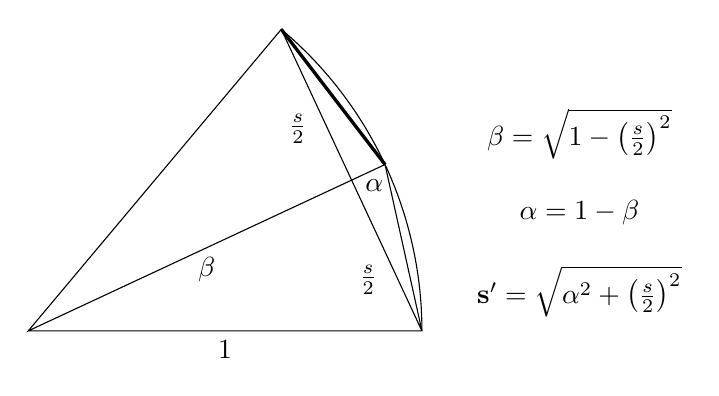
\begin{tikzpicture}[scale=5]
\draw (1,0) arc (0:50:1);
\draw (0,0) -- node[below] {1} ({cos(0)},{sin(0)}) -- ({cos(25)},{sin(25)}) -- node[pos=0.03,below] {$\alpha$} node[midway,below] {$\beta$}  (0,0) -- ({cos(50)},{sin(50)}) -- node[near start,below left] {$\frac{s}{2}$} node[near end, below left] {$\frac{s}{2}$} (1,0);
\draw[very thick] ({cos(50)},{sin(50)}) -- ({cos(25)},{sin(25)});
\draw (1.4,.5) node {$\beta = \sqrt{1-\left(\frac{s}{2}\right)^2}$};
\draw (1.4,.3) node {$\alpha= 1-\beta$};
\draw (1.4,.1) node {${\bf s'} = \sqrt{\alpha^2+\left(\frac{s}{2}\right)^2}$};
\end{tikzpicture}

\end{document}